%%
% This is an Overleaf template for presentations
% using the TUM Corporate Desing https://www.tum.de/cd
%
% For further details on how to use the template, take a look at our
% GitLab repository and browse through our test documents
% https://gitlab.lrz.de/latex4ei/tum-templates.
%
% The tumbeamer class is based on the beamer class.
% If you need further customization please consult the beamer class guide
% https://ctan.org/pkg/beamer.
% Additional class options are passed down to the base class.
%
% If you encounter any bugs or undesired behaviour, please raise an issue
% in our GitLab repository
% https://gitlab.lrz.de/latex4ei/tum-templates/issues
% and provide a description and minimal working example of your problem.
%%


\documentclass[
  english,            % define the document language (english, german)
  aspectratio=169,    % define the aspect ratio (169, 43)
  % handout=2on1,       % create handout with multiple slides (2on1, 4on1)
  % partpage=false,     % insert page at beginning of parts (true, false)
  % sectionpage=true,   % insert page at beginning of sections (true, false)
]{tumbeamer}
\usepackage{dingbat}

\usepackage{lmodern}
\usepackage{fontawesome}

\usepackage{tikz,dot2texi}
\usepackage{tikzsymbols}
\usepackage{tcolorbox}
\usepackage{lipsum}
\usepackage[
backend=biber,
style=authoryear,
]{biblatex}
\addbibresource{./aux/bib.bib}

\usetikzlibrary{mindmap}
% For adding shadows.
\usetikzlibrary{shadows}
% Extra arrows tips.
\usetikzlibrary{arrows.meta}
% Old arrows.
\usetikzlibrary{arrows}
% Automata.
\usetikzlibrary{automata}
% For more positioning options.
\usetikzlibrary{positioning}
% Creating chains of nodes on a line.
\usetikzlibrary{chains}
% Fitting node to contain set of coordinates.
\usetikzlibrary{fit}
% Extra shapes for drawing.
\usetikzlibrary{shapes}
\usetikzlibrary{trees,shapes,snakes}

% For markings on paths.
\usetikzlibrary{decorations.markings}
% For advanced calculations.
\usetikzlibrary{calc}
\usepackage{xcolor}
\setbeamertemplate{bibliography entry article}{}
\setbeamertemplate{bibliography entry title}{}
\setbeamertemplate{bibliography entry location}{}
\setbeamertemplate{bibliography entry note}{}

% load additional packages
\usepackage{booktabs}

% presentation metadata
\title{Parametrized Complexity}
\subtitle{Seminar: Advanced Algorithms}

\author{Lukas Retschmeier}

\institute{\theChairName\\\theDepartmentName\\\theUniversityName}
\date[03/02/2022]{February 3\textsuperscript{rd}, 2022}

\footline{\insertauthor~|~\insertshorttitle~|~\insertshortdate}
\newcommand*{\QEDA}{\hfill\ensuremath{\blacksquare}}
% macro to configure the style of the presentation
\TUMbeamersetup{
  title page = TUM tower,         % style of the title page
  part page = TUM toc,            % style of part pages
  section page = TUM toc,         % style of section pages
  content page = TUM more space,  % style of normal content pages
  tower scale = 0.8,              % scaling factor of TUM tower (if used)
  headline = TUM threeliner,      % which variation of headline to use
  footline = TUM infoline,         % which variation of footline to use
  % configure on which pages headlines and footlines should be printed
  headline on = {title page},
  footline on = {every page, title page=false},
}

% available frame styles for title page, part page, and section page:
% TUM default, TUM tower, TUM centered,
% TUM blue default, TUM blue tower, TUM blue centered,
% TUM shaded default, TUM shaded tower, TUM shaded centered,
% TUM flags
%
% additional frame styles for part page and section page:
% TUM toc
%
% available frame styles for content pages:
% TUM default, TUM more space
%
% available headline options:
% TUM empty, TUM oneliner, TUM twoliner, TUM threeliner, TUM logothreeliner
%
% available footline options:
% TUM empty, TUM default, TUM infoline


\begin{document}

\maketitle
\begin{frame}[c]{Classical Complexity Theory}
    \begin{itemize}   
        \item Usually aims for a polynomial-time (PTIME) algorithm
        \item For NP complete problems, we do not expect a PTIME algorithms
        \item \textbf{For Example: } $\mathtt{3SAT}$, $\mathtt{3COLORING}$, $\mathtt{CLIQUE}$, $\mathtt{VERTEX~COVER}$, ...
    \end{itemize}
    
    \begin{center}
    \textbf{But ... Can we say anything more about those problems?}
    \end{center}
\end{frame}


\begin{frame}[c]{Agenda: Our Plan for Today}
\begin{enumerate}
    \pause\item \textbf{Introduction and Definitions}
    \pause\item \textbf{Fixed Parameter (In)Tractibility \& $\omega$-Hardness}
    \pause\item \textbf{A Stronger Assumption: (S)ETH and Proving Lower Bounds}
\end{enumerate}
\end{frame}

\begin{frame}[c]{}
\begin{center}
    \textbf{Part I}
    
    \textit{Introduction and Definitions}
\end{center}
\end{frame}

\begin{frame}[c]{Ways to Cope with NP-Complete Problems}
\begin{center}
    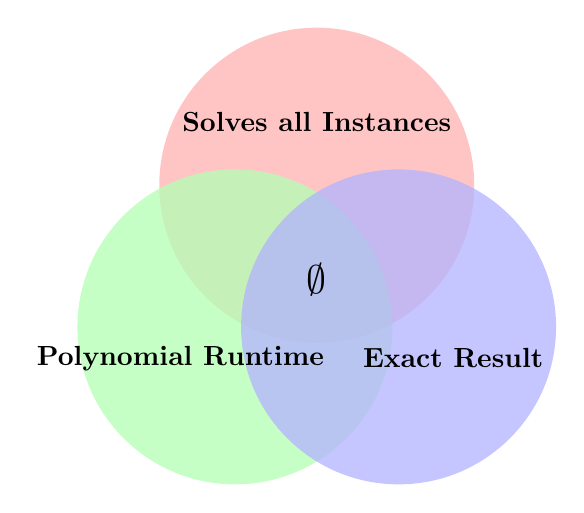
\begin{tikzpicture}
  \begin{scope}[blend mode = normal,opacity=0.75]
    \fill[red!30!white]   ( 90:1.2) circle (2);
    \fill[green!30!white] (210:1.2) circle (2);
    \fill[blue!30!white]  (330:1.2) circle (2);
  \end{scope}
  \node at ( 90:2)    {\textbf{Solves all Instances}};
  \node at ( 210:2)   {\textbf{Polynomial Runtime}};
  \node at ( 330:2)   {\textbf{Exact Result}};
  \node [font=\Large] {$\emptyset$};
\end{tikzpicture}

\end{center}
\end{frame}


\begin{frame}[c]{Ways to Cope with NP-Complete Problems}
\begin{columns}[c]
    \begin{column}{.48\textwidth}
\begin{center}
    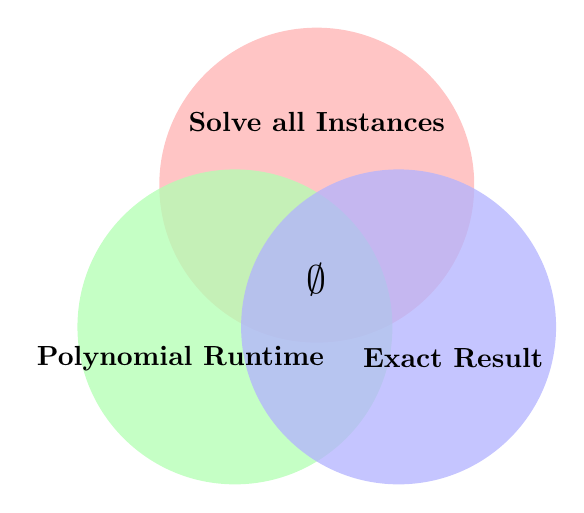
\begin{tikzpicture}
  \begin{scope}[blend mode = normal,opacity=0.75]
    \fill[red!30!white]   ( 90:1.2) circle (2);
    \fill[green!30!white] (210:1.2) circle (2);
    \fill[blue!30!white]  (330:1.2) circle (2);
  \end{scope}
  \node at ( 90:2)    {\textbf{Solve all Instances}};
  \node at ( 210:2)   {\textbf{Polynomial Runtime}};
  \node at ( 330:2)   {\textbf{Exact Result}};
  \node [font=\Large] {$\emptyset$};
\end{tikzpicture}
\end{center}
\end{column}
    \begin{column}{.48\textwidth}
    We must give up at least one:
    
    \begin{itemize}
        \pause\item \textbf{Exactness: } Approximation Algorithms
        \pause\item \textbf{Polynomial Runtime: } Exact Exponential Time Algorithms 
        \pause\item \textbf{Generality: } \textcolor{blue}{\textbf{FPT Algorithms}}
    \end{itemize}
    \end{column}
\end{columns}
\end{frame}



\begin{frame}[c]{Parametrized Complexity}
\begin{itemize}
    \item \textit{Parametrized Complexity} can be seen as a \textit{2-Dimensional} complexity analysis
    \item Looking deep into the \textit{nature of the problem} to find some hidden (in)-feasibility
    \begin{itemize}
        \item Graph of small size?
        \item Planar Graph? A Tree?
        \item Forbidden Minor?
        \item Regular? Degree-Bounded?
        \item Bipartite? Chordal?\footnote{A State-of-the-art collection: \url{https://www.graphclasses.org/}}
        \item ...
    \end{itemize}
\end{itemize}
\end{frame}

\begin{frame}[c]{The Idea Behind: \textit{Bar Fight Prevention}}

\begin{exampleblock}{The Problem}
Owning a Bar is very difficult! You already know that some people might fight so you prevent certain trouble makersfrom entering. \textbf{How many do you have to block to resolve all conflicts?}
\end{exampleblock}

\begin{center}
    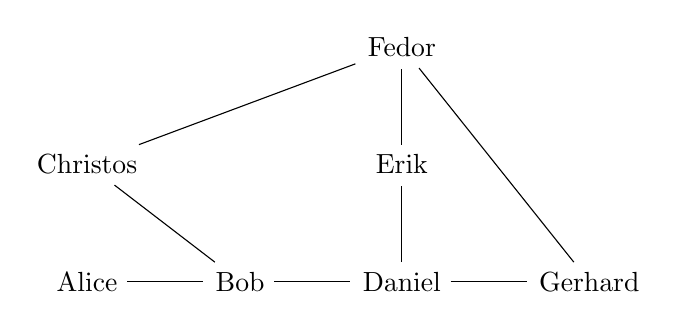
\begin{tikzpicture}[>=stealth', shorten >=1pt, auto,
    node distance=1cm, scale=1, 
    transform shape, align=center, 
    state/.style={circle, draw, minimum size=1cm,thick}]
		   \node[] (D) {Daniel};
		    \node[right=of D] (G) {Gerhard};
		    \node[left=of D] (B) {Bob};
		    \node[above=of B,left=of B] (A) {Alice};
		    \node[above=of D] (E) {Erik};
		    \node[above=of E] (F) {Fedor};
		    \node[above=of D,left=of F,right=of A,left=of E,above=of A] (C) {Christos};
	    
   	    	\path (A) edge (B);
    		\path (B) edge (C);
   	    	\path (B) edge (D);
    		\path (D) edge (E);
    		\path (D) edge (G);
    		\path (G) edge (F);
    		\path (E) edge (F);
    		\path (C) edge (F);
    \end{tikzpicture}
\end{center}
\end{frame}

\begin{frame}[c]{The Idea Behind: \textit{Bar Fight Prevention}}
\begin{center}
    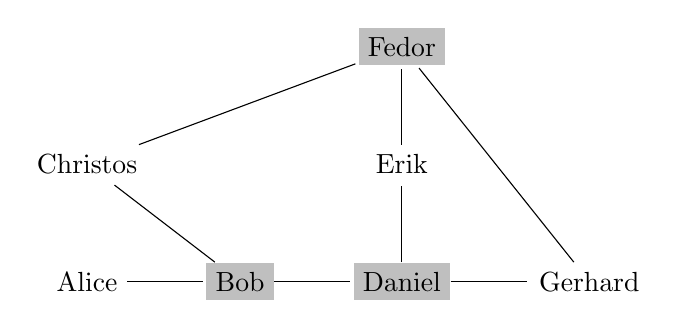
\begin{tikzpicture}[>=stealth', shorten >=1pt, auto,
    node distance=1cm, scale=1, 
    transform shape, align=center, 
    state/.style={circle, draw, minimum size=1cm,thick}]
		   \node[fill=lightgray] (D) {Daniel};
		    \node[right=of D] (G) {Gerhard};
		    \node[fill=lightgray,left=of D] (B) {Bob};
		    \node[above=of B,left=of B] (A) {Alice};
		    \node[above=of D] (E) {Erik};
		    \node[fill=lightgray,above=of E] (F) {Fedor};
		    \node[above=of D,left=of F,right=of A,left=of E,above=of A] (C) {Christos};
	    
   	    	\path (A) edge (B);
    		\path (B) edge (C);
   	    	\path (B) edge (D);
    		\path (D) edge (E);
    		\path (D) edge (G);
    		\path (G) edge (F);
    		\path (E) edge (F);
    		\path (C) edge (F);
    \end{tikzpicture}
    
    
\end{center}

    \pause\begin{exampleblock}{Observation}
        Removing \textit{Fedor}, \textit{Daniel} and \textit{Bob} resolves all conflicts.
    \end{exampleblock}
    \pause \textbf{Assuming 1.000 guests: $2^{1000}\approx 1.07\cdot10^{301}$}
    \textcolor{red}{\textbf{Absolutely infeasible}}
    
\end{frame}

\begin{frame}{Restricting the Problem}
    \textbf{Question: } What happens if you just have a budget of $k$-people you would like to refuse?
    \\~
    
    \begin{center}
    
    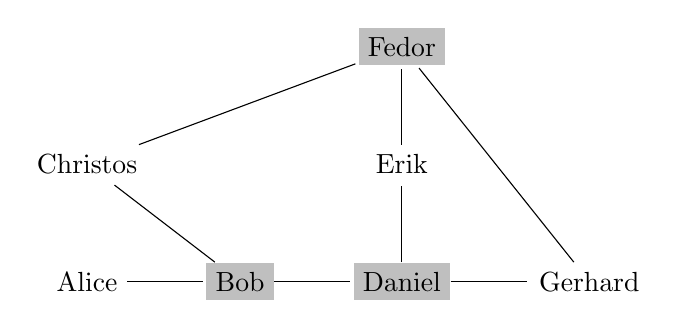
\begin{tikzpicture}[>=stealth', shorten >=1pt, auto,
    node distance=1cm, scale=1, 
    transform shape, align=center, 
    state/.style={circle, draw, minimum size=1cm,thick}]
		   \node[fill=lightgray] (D) {Daniel};
		    \node[right=of D] (G) {Gerhard};
		    \node[fill=lightgray,left=of D] (B) {Bob};
		    \node[above=of B,left=of B] (A) {Alice};
		    \node[above=of D] (E) {Erik};
		    \node[fill=lightgray,above=of E] (F) {Fedor};
		    \node[above=of D,left=of F,right=of A,left=of E,above=of A] (C) {Christos};
	    
   	    	\path (A) edge (B);
    		\path (B) edge (C);
   	    	\path (B) edge (D);
    		\path (D) edge (E);
    		\path (D) edge (G);
    		\path (G) edge (F);
    		\path (E) edge (F);
    		\path (C) edge (F);
    \end{tikzpicture}
\end{center}
    
    \\~
    \pause \textbf{Assuming 1.000 guests and $k=10$: $\binom{1000}{10}\approx2.62\cdot10^{23}$}
    \textcolor{red}{\textbf{Still pretty infeasible}}
\end{frame}

\begin{frame}{Can we do better?}

    \begin{exampleblock}{Observation}
    Someone fighting with at least $k+1$ other guests must be refused, because otherwise\textbf{all other $k+1$} guests must be refused exceeding our budget
    \end{exampleblock}
    
    \begin{center}
    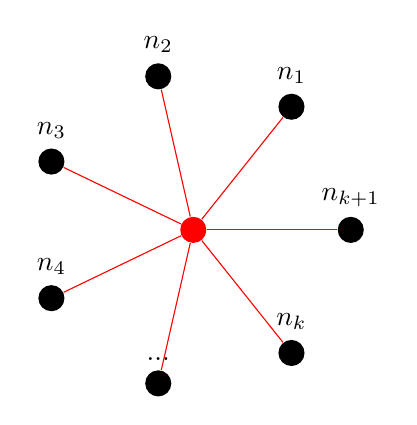
\begin{tikzpicture}
      \node[circle,fill=red] at (360:0mm) (center) {};
    \foreach \n in {1,...,4}{
        \node[circle,fill=black,label=$n_\n$] at ({\n*360/7}:2cm) (n\n) {};
        \draw[red] (center)--(n\n);
    }
        \node[circle,fill=black,label={$n_{k}$}] at ({6*360/7}:2cm) (n6) {};
        \draw[red](center)--(n6);
        \node[circle,fill=black,label={$n_{k+1}$}] at ({7*360/7}:2cm) (n7) {};
        \draw[red](center)--(n7);
        \node[circle,fill=black,label={$...$}] at ({5*360/7}:2cm) (n5) {};
        \draw[red](center)--(n5);
    \end{tikzpicture}
    \end{center}
\end{frame}

\begin{frame}[c]{Kernelization I}
\begin{itemize}
    \item $\mathtt{max}_{\mathtt{deg}} \leq k$
    \item Rejecting a guest will now resolve at most k conflicts
    \item We are allowed to remove \textbf{at most} $k$ guests each having at most $k$ conflicts
    \item If $ > k^2$ conflicts remaining: No way to resolve all: \textbf{Refuse Instance}
\end{itemize}
\begin{center}

$\binom{2k^2}{k} \leq \binom{200}{10} \approx 2.24\cdot 10^{16}$


\hbox{
\textcolor{gray}{\textbf{Feasible, but still ...}}
}
\end{center}
   \pause\textbf{Note: }This technique is called \textit{Kernelization}. 
\end{frame}

\begin{frame}[c]{Kernelization II: Improvement}

    \begin{exampleblock}{Observation}
    If $deg(n) = 1$ refuse $N[v]$ and decrease $k$ 
    \end{exampleblock}
    
\begin{columns}[T] % align columns
    \begin{column}{.48\textwidth}
 \begin{center}
    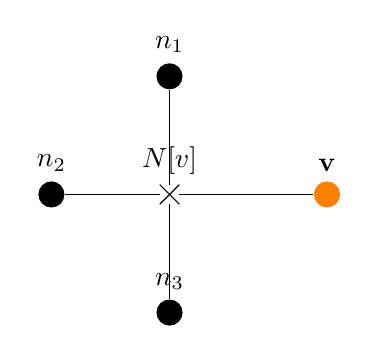
\begin{tikzpicture}
      \node[circle,fill=red,cross out=red,draw,label={$N[v]$}] at (360:0mm) (center) {};
    \foreach \n in {1,...,3}{
        \node[circle,fill=black,label=$n_\n$] at ({\n*360/4}:1.5cm) (n\n) {};
        \draw (center)--(n\n);
    }
        \node[circle,fill=orange,label={$\mathbf{v}$}] at ({4*360/4}:2cm) (n7) {};
        \draw (center)--(n7);
    \end{tikzpicture}
    \end{center}
\end{column}%
\begin{column}{.48\textwidth}
\textbf{Analysis}
\begin{itemize}
    \item Degree now bounded by $1 < \mathtt{deg}(v) <= k$
    \item $\binom{k^2}{k} \leq \binom{100}{10} \approx 1.73  \cdot 10^{13}$
    \item \textbf{Even Better!} 
\end{itemize}
\end{column}%
\end{columns}
\end{frame}

\begin{frame}{A Different Approach: Bounded Search Trees}
\begin{alertblock}{Crucial Observation}
Every conflict \textit{must} be resolved. 

$\Rightarrow$ For every conflicting pair \textbf{at least one must be refused }\footnote{This also leads to  2-approximation algorithm! (See: \cite[Ch. 35.1]{CLRS})}

\end{alertblock}

\begin{columns}[T] % align columns
    \begin{column}{.48\textwidth}
    \begin{center}
            \pause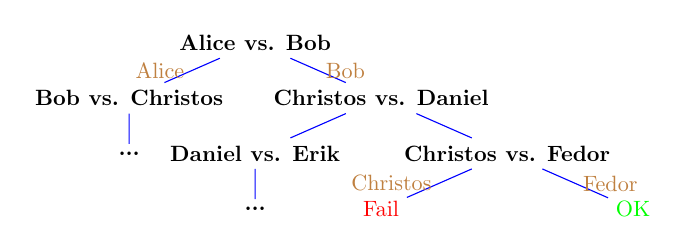
\begin{tikzpicture}[scale=0.8,transform shape]
            \node {\textbf{Alice vs. Bob}} [sibling distance = 4cm, level distance = 25pt]
                child {node {\textbf{Bob vs. Christos}}
                    child {node {\textbf{...} }}
                edge from parent [blue] node [left, brown] {Alice} 
                }
                child {node {\textbf{Christos vs. Daniel}}
                        child {node {\textbf{Daniel vs. Erik}}
                            child {node {\textbf{...}}}
                        }
                        child {node [sibling distance=1cm] {\textbf{Christos vs. Fedor}}
                                child {node {\textcolor{red}{Fail}}
                                    edge from parent [blue] node [left, brown] {Christos}
                                }
                                child {node {\textcolor{green}{OK}}
                                    edge from parent [blue] node [right, brown] {Fedor}
                                }
                        }
                edge from parent [blue] node [right, brown] {Bob}
                };
            \end{tikzpicture}
        \end{center}
    \end{column}
   \pause\begin{column}{.48\textwidth}
  \begin{center}
    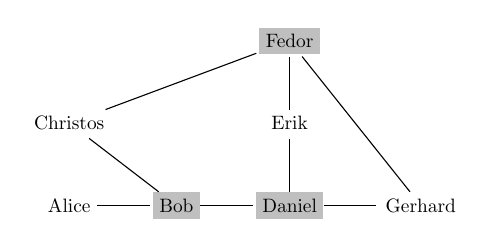
\begin{tikzpicture}[>=stealth', shorten >=1pt, auto,
    node distance=1cm, scale=0.7, 
    transform shape, align=center, 
    state/.style={circle, draw, minimum size=1cm,thick}]
		   \node[fill=lightgray] (D) {Daniel};
		    \node[right=of D] (G) {Gerhard};
		    \node[fill=lightgray,left=of D] (B) {Bob};
		    \node[above=of B,left=of B] (A) {Alice};
		    \node[above=of D] (E) {Erik};
		    \node[fill=lightgray,above=of E] (F) {Fedor};
		    \node[above=of D,left=of F,right=of A,left=of E,above=of A] (C) {Christos};
	    
   	    	\path (A) edge (B);
    		\path (B) edge (C);
   	    	\path (B) edge (D);
    		\path (D) edge (E);
    		\path (D) edge (G);
    		\path (G) edge (F);
    		\path (E) edge (F);
    		\path (C) edge (F);
    \end{tikzpicture}
\end{center}
    \end{column}
\end{columns}
\end{frame}


\begin{frame}[c]{Final Runtime Using Branching}

\begin{itemize}

\item We branch into \textbf{two sub-branches} and always \textbf{decrease k by one}.
\pause \item Traversing the graph yields  $\mathcal{O}(m+n)$.
\pause \item Recall $ m \leq \frac{nk}{2}$ after our preciously discussed pre-processing procedure
\end{itemize}

\textbf{So we finally  get: }

$$ \mathcal{O}(2^k \cdot n \cdot k)$$ 

For $n = 1.000$ and $k = 10$: $2^{10} \cdot 1.000 \cdot 10 = 10.240.000$ \dSmiley

\end{frame}

\begin{frame}[c]{Parametrized Problem}
\textbf{Main Idea:} Instead of expressing the running time as a function $T(n)$ of n, we express it as a function $T(N,k)$ of the input size $n$ and \textit{some} parameter $k$ of the input.


\begin{block}{Definition 1: Parametrized Problem}
A parametrized problem is a $L\subseteq\Sigma^*\times N$ ($\Sigma$ finite fixed alphabet) for an instance $(x,k)\in \Sigma^*\times \mathrm{N}$, where k is called the \textcolor{orange}{parameter}.
\end{block}
\textbf{Examples for a parameter k:}
\begin{itemize}
    \item size k of a $\mathtt{VERTEX COVER}$
    \item size k of a $\mathtt{INDEPENDENT SET}$
    \item Treewidth k of a given graph
\end{itemize}
\end{frame}


\begin{frame}[c]{The Class FPT}

\begin{block}{Definition 2: Fixed-Parameter Tractable}
A parametrized problem $L\subseteq\Sigma^*\times\mathbb{N}$ is called \textit{fixed-parameter tractable (FPT)} if there exists an algorithm A (called a \textit{fixed-parameter algorithm}), a computable function $f:\mathbb{N} \rightarrow \mathbb{N}$ and a constant c such that, given $(x,k) \in \Sigma^* \times \mathbb{N}$, the algorithm \mathcal{A} correctly decides whether $(x,k) \in L$ in time bounded by $f(k) \cdot |(x,k)|^c$. The complexity class containing all fixed-parameter tractable problems is called \textcolor{blue}{FPT}.
\end{block}

\textbf{Note: } We often omit the polynomial-factor and rewrite the running time simply as $\mathcal{O}^*(f(k))$ 
\end{frame}

\begin{frame}[c]{The Class XP}

\begin{block}{Definition 3: Slice-Wise Polynomial}
A parametrized problem $L\subseteq \Sigma^* \times \mathbb{N}$ is called \textit{slice-wise polynomial} (XP) if there exists an algorithms \mathcal{A} and two computable functions $f,g:\mathbb{N}\rightarrow \mathbb{N}$ such that, given $(x,k) \in \Sigma^* \times \mathbb{N}$, the algorithm \mathcal{A} correctly decides whether $(x,k) \in L$ in time bounded by $f(k)\cdot|(x,k)|^{g(k)}$. The complexity class containing all slice-wise polynomial problems is called XP. 

\end{block}

\begin{alertblock}{XP vs FPT}
The class XP allows algorithms of the form $f(k) \cdot n^{g(k)}$ in contrast to FPT which tries to fix a polynomial constant c: $f(k)\cdot |(x,)|^c$. 

it can be shown: $FPT \subset XP$ by diagnolization.
\end{alertblock}
\end{frame}

\begin{frame}[c]{Vertex Cover}
\begin{itemize}
    \item The attentive listener might already have noticed that the introductory problem presented equals the NP-Complete $\mathtt{VERTEX~COVER}$ problem!
\end{itemize}

\begin{tcolorbox}[colback=green!5,colframe=green!40!black,title=$\mathtt{MIN~VERTEX~COVER}$ (\cite{Cygan2015})]
\begin{columns}[T] % align columns
    \begin{column}{.18\textwidth}
    \\~
    
    \textbf{Input:}\\
    \textbf{Question:}
    \end{column}
    \begin{column}{.78\textwidth}
    \\~
    
    Graph G and an Integer k\\
    Does there exist a set $S$ of vertices of size at most k s.t. $G - S$ is edgeless?
    \\~
    
   \textit{In other words: Is it possible to cover all edges of $G$ with at most $k$ vertices?}
    % https://www.cs.bme.hu/~dmarx/papers/marx-tractability-slides.pdf
    \end{column}
 \begin{center}
 \end{center}
 \end{columns}
\end{tcolorbox}
\end{frame}

\begin{frame}[c]{Outlook: Advanced Algorithmic Techniques}
\begin{columns}[c] % align columns
\begin{column}{.48\textwidth}
    \begin{center}
        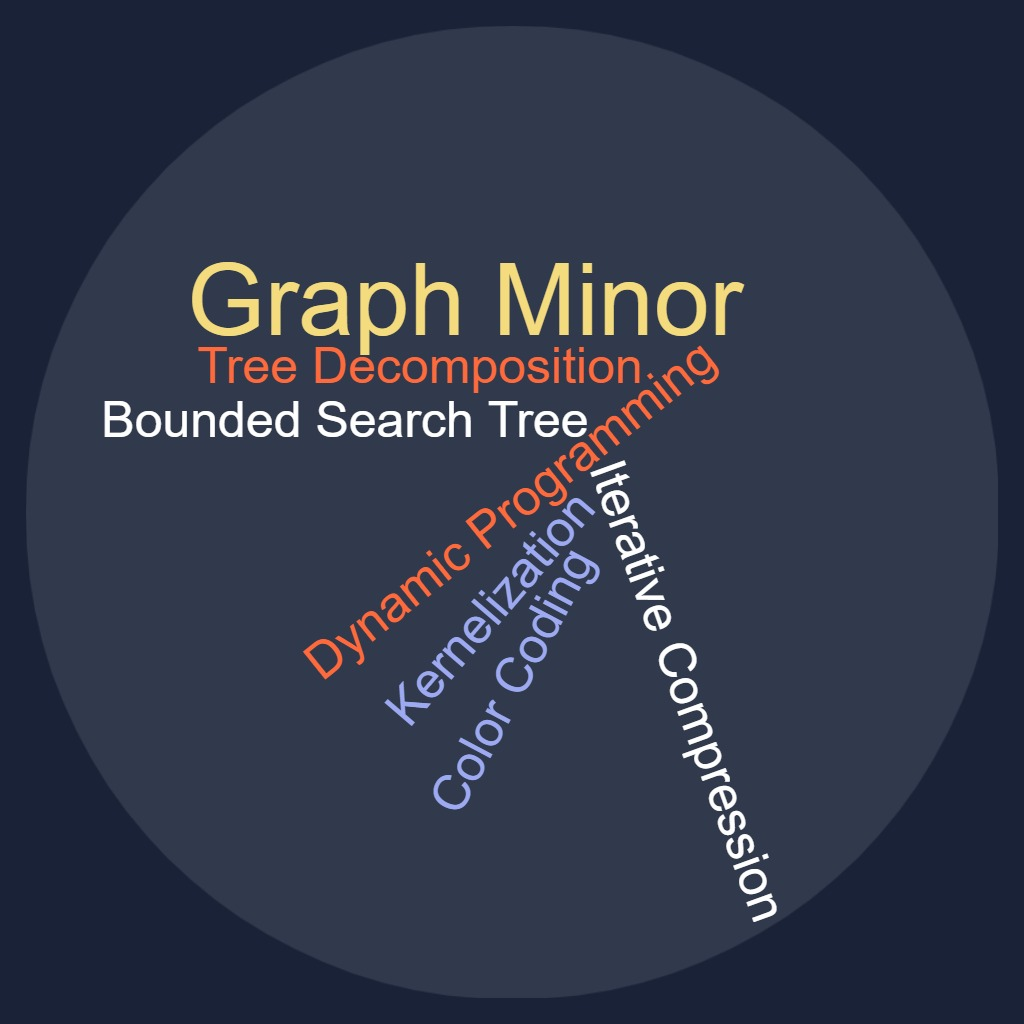
\includegraphics[scale=0.15]{img/wordcloud.jpg}
    \end{center}
\end{column}
\begin{column}{.48\textwidth}
    \begin{itemize}
        \item There exists many techniques to deduce fast FPT algorithms.
        \item \textit{PACE} challenges competitors to solve as many very hard instances as possible: \url{https://pacechallenge.org/}
    \end{itemize}
\end{column}
\end{columns}
\end{frame}

\begin{frame}[c]{Key Takeaways I}
\begin{center}
\begin{quote}
    If there would be just three things, you should take away...
\end{quote}
\begin{itemize}
    \pause\item Problems that are only exponential in a fixed parameter k while polynomial to the input size are called \textbf{Fixed-Parameter Tractable}
    \pause\item Uses additional information or properties about a specific instance of a problem.
    \pause\item There exists many different algorithmic techniques to obtain different FPT algorithms.
\end{itemize}
\end{center}
\end{frame}
\begin{frame}[c]{}
\begin{center}
    \textbf{Part II: Fixed Parameter (\textcolor{red}{In})Tractibility \& $w$-Hardness}
    
    \textit{Stepping towards lower-bounds for FPT}
    
\end{center}
\end{frame}

\begin{frame}[c]{Parametrized Hardness}

\pause\textbf{By Now: } Denote $\omega[1]$ as problems that might not expose a FPT algorithm. 

\pause\textbf{Goal:} A theory of Intractibility for Parametrized Problems
\begin{center}
    \begin{table}[]
    \begin{tabular}{@{}lll@{}}
     \topline
     & \textbf{NP-Hardness} & \textbf{W[1]-Hardness} \\
     \midrule
     \pause\textbf{Objects of Study} & "Classical" $L\subseteq \{0,1\}^*$ & "Parametrized" $L\subseteq \{0,1\}^* \times \mathbb{N}$  \\
     \pause\textbf{Tractibility} & PTIME & FPT \\
     \pause\textbf{Hardness Assumption} & $\texttt{SAT} \notin \texttt{PTIME} $ & $ \texttt{CLIQUE}_k \notin \texttt{FPT} $ \\
     \pause\textbf{Reductions} & Poly-Time Karb Reductions & {\color{green}{FPT Reductions}}  \\ \bottomrule
    \end{tabular}
\end{table}
\end{center}
\end{frame}


\begin{frame}[c]{Parametrized Reductions}
\begin{block}{Definition 4: Parametrized Reduction (\cite[Def 13.1]{Cygan2015})}
Let $A,B\subseteq \Sigma^*\times\mathbb{N}$ two parametrized problems. A \textit{Parametrized Reduction} from A to B is an algorithm that, given an instance $(x,k)$ of A, outputs an instance $(x', k')$ of B such that
\begin{itemize}
    \item $(x,k)$ is a \textcolor{gray}{yes instance} of A \textbf{iff} $(x',k')$ is a \textcolor{gray}{yes instance} of B \\
    \item $k' \leq g(k)$ for some computable function $g$
    \item the running time is $f(k)\cdot |x|^{\mathcal{O}(1)}$
\end{itemize}
\end{block}

\end{frame}

\begin{frame}[c]{Parametrized Reductions}
\begin{center}
\begin{block}{Theorem 1: Central Property of Parametrized Reductions (\cite[Th. 13.2]{Cygan2015})}{If there is a Parametrized Reduction from L to Q and Q is FPT, then L is FPT as well. }
\end{block}
\end{center}
\textbf{Proof: Follows from definition} 
\begin{itemize}
    \pause\item Suppose Q can be solved in $\mathtt{FPT\-TIME}$~ $f(l) \cdot |y|^c$ ) and the reduction $L \leq_{\mathtt{FPT}} Q$ takes time $g(k) \cdot |x|^d$
    \pause\item Then L solves in $f(h(k)) \cdot (g(k) \cdot |x|^d)^c$ as  l bounded by $l \leq h(k)$ (Property II) and the instance can not be larger then the duration of the reduction
    \item The final runtime only exponential in k and polynomial in |x| and hence FPT \QEDA
    \end{itemize}
\end{frame}

\begin{frame}[c]{Parametrized Reductions}
\begin{center}
\begin{block}{Theorem 2: Transitivity \cite[Th. 13.3]{Cygan2015}}
If there are Parametrized Reductions from  L to Q and from Q to T, then there is a Parametrized Reduction from L to T.
\end{block}
    \textbf{Proof: Omitted. Again directly from the Definition}
\end{center}
\end{frame}

\begin{frame}[c]{Towards a New Hierarchy}
\begin{center}
\begin{block}{(Rather Informal) Definition: The class $\omega[1]$}
$\omega[1] := [\mathtt{CLIQUE}_k]^{\mathtt{FPT}}$ (All problems FPT-reducible to $\mathtt{CLIQUE}_k$)
\end{block}
\begin{itemize}
    \pause\item Problem Q is $\omega[1]$-hard iff $\mathtt{CLIQUE}_k$ reduces to it.
    \pause\item $\mathtt{FPT} \subseteq \omega[1]$
    \pause\item $P = NP \Rightarrow \mathtt{FPT} = \omega[1]$
    \pause\item If $\omega[1]$-hard problem is \mathtt{FPT} then also collapse $\mathtt{FPT} =  \omega[1]$
\end{itemize}
\end{center}
\end{frame}

\begin{frame}[c]{Recap: Independent Set}
\begin{center}
\begin{tcolorbox}[colback=green!5,colframe=green!40!black,title=$\mathtt{INDEPENDENT~SET}$ (See \cite{Cygan2015})]
\begin{columns}[T] % align columns
    \begin{column}{.18\textwidth}
    \\~
    
    \textbf{Input:}\\
    \textbf{Question:}
    \end{column}
    \begin{column}{.78\textwidth}
    \\~
    
    Graph G and integer k\\
    Does G has an independent set of size k?
    \\~
    
   \textit{In other words: Is there a vertex-set $S$ of size $k$  that are non-adjacent?}
    \end{column}
 \end{columns}
\end{tcolorbox}

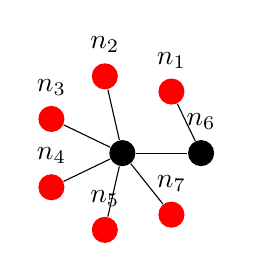
\begin{tikzpicture}
      \node[circle,fill=black] at (360:0mm) (center) {};
    \foreach \n in {2,...,5}{
        \node[circle,fill=red,label=$n_\n$] at ({\n*360/7}:1cm) (n\n) {};
        \draw (center)--(n\n);
    }
        \node[circle,fill=red,label={$n_1$}] at ({360/7}:1cm) (n1) {};
        \node[circle,fill=red,label={$n_7$}] at ({6*360/7}:1cm) (n6) {};
        \draw (center)--(n6);
        \node[circle,fill=black,label={$n_6$}] at ({7*360/7}:1cm) (n7) {};
        \draw (n1) -- (n7);
        \draw (center)--(n7);
\end{tikzpicture}
\end{center}
\end{frame}

\begin{frame}[c]{A First Trivial Reduction: $\mathtt{CLIQUE}_k \leq_{\mathtt{FPT}} \mathtt{IS}_k$}
\begin{center}

\begin{itemize}
    \pause\item It is known: Graph G has $\mathtt{IS}$ of size k if and only if $G^{-1}$ has a $\mathtt{CLIQUE}$ of size k.
    \pause\item Therefore: $(G, k) \longrightarrow (G^{-1}, k)$ directly gives the desired reduction (Even in PTIME!).
\end{itemize}
\end{center}
\end{frame}

\begin{frame}[c]{Why Standard Reductions Not Always Work:  $\mathtt{VC}_k \leq_{\mathtt{FPT??}} \mathtt{IS}_k$}
\begin{center}

\begin{itemize}
    \pause\item Again, it is known: X is a $\mathtt{VC}$ if and only if $G - X $ is an $\mathtt{IS}$.
    \pause\item Therefore: $(G, k) \longrightarrow (G, n - k)$ gives indeed a reduction,  \textbf{but} %TODO Really? 
    \pause\item The parameter k is not bounded any more just by k!
\end{itemize}
\end{center}
\end{frame}



\begin{frame}[c]{Multicolored Clique}
\begin{center}
\begin{tcolorbox}[colback=green!5,colframe=green!40!black,title=\textrm{MULTICOLORED~CLIQUE~(PARTITIONED~CLIQUE) \cite[p. 428]{Cygan2015}}]
\begin{columns}[T] % align columns
    \begin{column}{.18\textwidth}
    \\~
    
    \textbf{Input:}\\
    \textbf{Question:}
    \end{column}
    \begin{column}{.78\textwidth}
    \\~
    
    Graph G, integer k, partition $(V_1, ...V_k)$\\
    Does G has a $k$-Clique containing \textbf{exactly} one vertex from each set $V_i$?
    \end{column}
 \end{columns}
\end{tcolorbox}
\end{center}
\end{frame}

\begin{frame}[c]{$\mathtt{CLIQUE}_k \leq_{\mathtt{FPT}} \mathtt{MULTICOLORED~CLIQUE}_k$}
\textbf{Idea: } Distribute a Clique to k partitions
    \begin{center}
        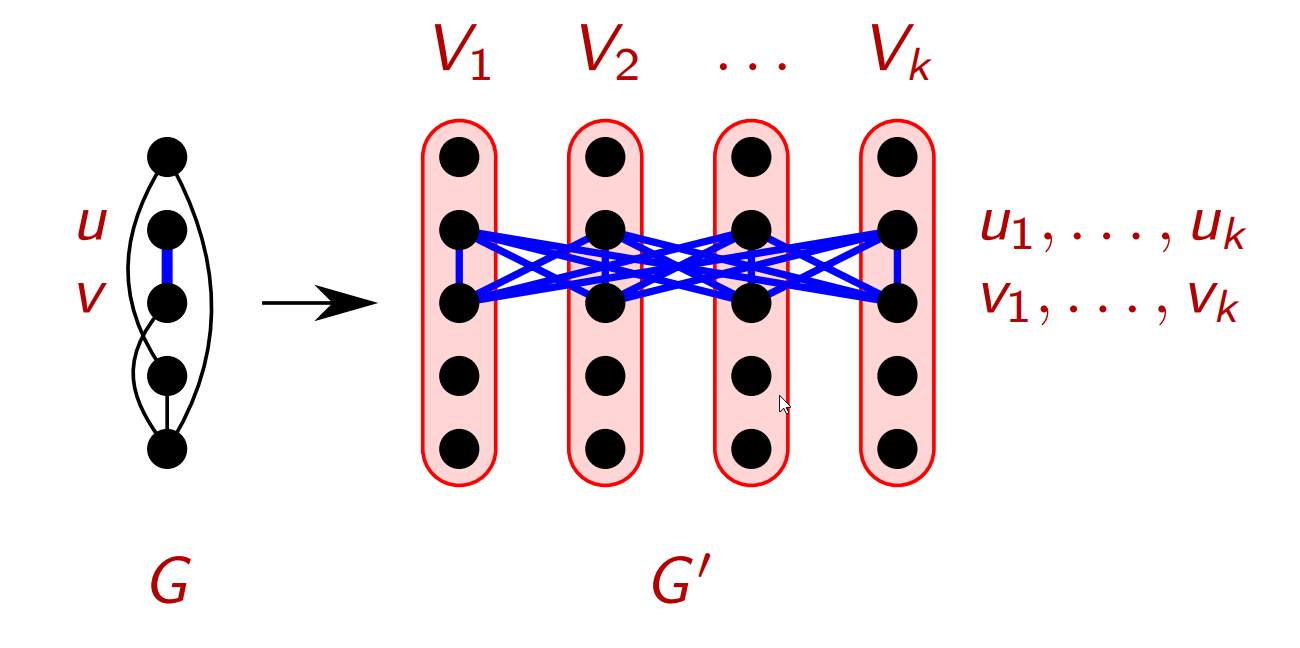
\includegraphics[scale=0.17]{img/Unbenannt.png}
    \end{center}
\textbf{Proof} 
\begin{itemize}
    \item $\mathtt{CLIQUE}_k \Rightarrow \mathtt{M\-CLIQUE}_k$: Distribute original clique to partitions
    \item $\mathtt{M\-CLIQUE} \Rightarrow \mathtt{CLIQUE}_k$: Project them back to a set of vertices of G
\end{itemize}
\textbf{Therefore: }$(G,k) \longrightarrow (G',k')$ is a FPT reduction. 
\end{frame}

\begin{frame}[c]{Notes}
\begin{itemize}
\item  For proofing $\omega[1]$ hardness, it is often useful to start with a $\mathtt{MULTICOLORED~CLIQUE}$
\item Similar, there is a FPT reduction from $\mathtt{INDEPENDENT~SET} \leq_{\mathtt{FPT}} \mathtt{MULTICOLORED~INDEPENDENT~SET}$
\end{itemize}
\end{frame}


\begin{frame}[c]{Dominating Set}

\begin{center}
\begin{tcolorbox}[colback=green!5,colframe=green!40!black,title=$\mathtt{DOMINATING~SET}$ (\cite{Cygan2015})]
\begin{columns}[T] % align columns
    \begin{column}{.18\textwidth}
    \\~
    
    \textbf{Input:}\\
    \textbf{Question:}
    \end{column}
    \begin{column}{.78\textwidth}
    \\~
    
    Graph G and Integer k\\
    Is there $X$ of size $k$ s.t. $N[X] = V(G)$?
    
    \end{column}
 \end{columns}
 
\\~

Where we denote $N[X]$ as the \textbf{close neighborhood} of $X$
\end{tcolorbox}
\end{center}

\textbf{Corollary: } $\mathtt{DOMINATING~SET}$ is $\omega[1]$-hard and $\omega[2]$-complete  

\end{frame}

\begin{frame}{Intuition About Differences of $\omega[1]$ and $\omega[2]$}

Formulating $\mathtt{CLIQUE}$ and $\mathtt{DOMINATING~SET}$ in logical terms \footnote{More precisely: Monadic Second-Order-Logic of Graphs}

\begin{center}
\begin{itemize}
    \item X is a $\mathtt{CLIQUE}$ iff $$\forall_{\mathrm{(u,v) \notin G}}: u \notin X \lor v \notin X $$
%    (Every non-edge, not both are in the Clique
    \item X is a $\mathtt{DOMINATING~SET}$ iff $$\forall u \exists v: v \in X \land (u,v) \in E(G) $$
\end{itemize}
\end{center}

\textbf{Recall: } The Polynomial Hierarchy also defined via quantifiers. 

\textbf{Maybe something similiar applies also in the FPT case?}

\end{frame}

\begin{frame}{Intuition About Differences of $\omega[1]$ and $\omega[2]$}
\begin{columns}[T] % align columns
    \begin{column}{.5\textwidth}
    sdsf
    \end{column}
    \begin{column}{.5\textwidth}
    lkj
    \end{column}
\end{columns}

  \begin{tikzpicture}[level/.style={sibling distance=15mm/#1}, scale = 0.8]
    \node [circle,draw] (z){$\land$}
    child {node [circle,draw] (a) {$\neg\land$}
        child {node [] (b) {$x_1$}
        }
  }
  child {node [circle,draw] (j) {$\neg \land$}
        child {node [] (c) {$x_2$}
        }
}
  child {node [circle,draw] (w) {$\neg \land$}
        child {node [] (d) {$x_3$}
        }
  }
  child {node [circle,draw] (q) {$\neg \land$}
        child {node [] (e) {$x_4$}
        }
  }
  child {node [circle,draw] (r) {$\neg \land$}
        child {node [] (f) {$x_5$}
        }
  }
  \draw (b) -- (c)
  
  \end{tikzpicture}
\end{frame}

\begin{frame}{Quick Outlook: Weighted Circuit Satisfiability}

\begin{tcolorbox}[colback=green!5,colframe=green!40!black,title=$\mathtt{WEIGHTED~CIRCUIT~SATISFIABILITY (WCS)}$ (\cite{Cygan2015})]
\begin{columns}[T] % align columns
    \begin{column}{.18\textwidth}
    \\~
    
    \textbf{Input:}\\
    \textbf{Question:}
    \end{column}
    \begin{column}{.78\textwidth}
    \\~
    
    Circuit C and Integer k\\
    
    Is there a satisfying valuation of the input \textbf{with exactly k ones}?
    
    \end{column}
 \end{columns}

\end{tcolorbox}


\textbf{Definition: } $\omega[t] := $ Problems FPT-Reducible to $\mathtt{WCS}$ for circuits of 
\begin{itemize}
    \item Constant Depth and
    \item weft at most t
\end{itemize}

\end{frame}


%TODO:: 
%https://wuecampus2.uni-wuerzburg.de/moodle/pluginfile.php/1564087/mod_resource/content/3/vl09-part2-printerversion.pdf
\begin{frame}[c]{Summary FPT Reductions\footnote{(Comp. \cite{fptland})}}
    \begin{center}
        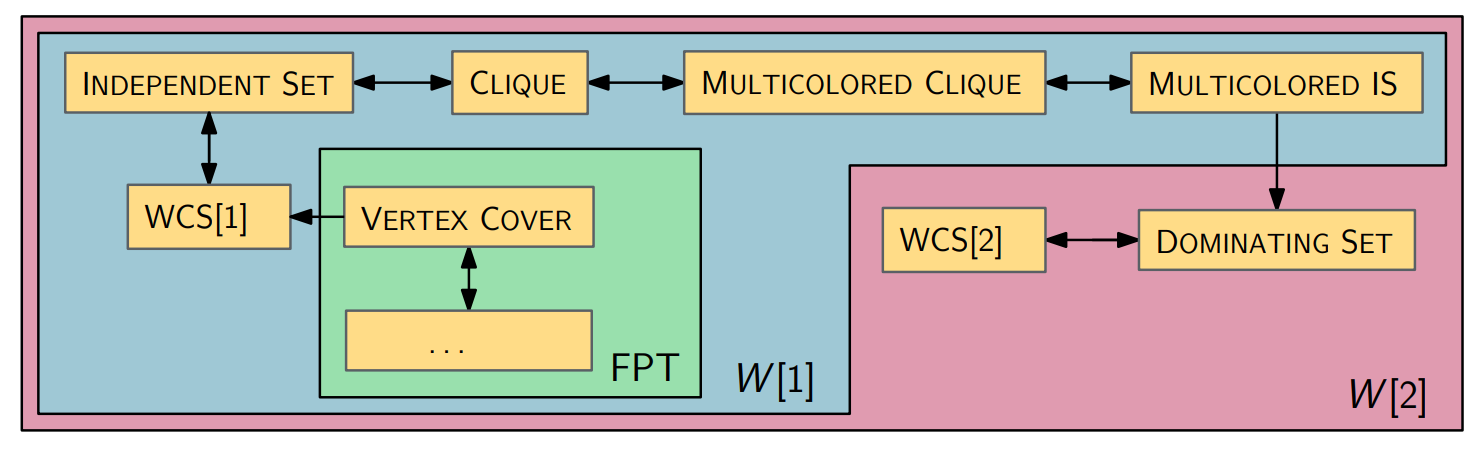
\includegraphics[scale=0.3]{img/landscape.png}
    \end{center}
\end{frame}

\begin{frame}[c]{Key Takeaways II}
\begin{center}
\begin{quote}
    If there would be just three things, you should take away...
\end{quote}
\begin{itemize}
    \item $\mathtt{Vertex Cover} \in \mathtt{FPT}$,  $\mathtt{Clique}_k \in \omega[1]$ and  $\mathtt{Dominating Set} \in \omega[2]$
    \item The class NP splits up into a hierarchy of more  $\omage[i]$ classes
\end{itemize}
\end{center}
\end{frame}

\begin{frame}[c]{}
\begin{center}
    \textbf{Part III: A Stronger Assumption: The (Strong) Expontential Time Hypothesis}
    
    \textit{Proving Lower Bounds For Subexponential Time}
\end{center}
\end{frame}


\begin{frame}[c]{Why We Need a New a Assumption}

\begin{center}
We already know for the \textbf{Vertex Cover} problem:

\begin{enumerate}
    \pause\item $2^n \cdot poly(n)$ by brute-forcing all sets
    \pause\item $2^k \cdot poly(n)$ by \textit{branching}
\end{enumerate}

But for example: \textbf{Planar Vertex Cover} can be solved in 
\begin{enumerate}
    \pause\item $2^{\mathcal{O}(n^{1/3})}$ by TODO
    \pause\item $2^{\mathcal{O}(k^{1/3})} \cdot n^{\mathcal{O}(1)} $ by TODO
\end{enumerate}
\end{center}

\end{frame}
\begin{frame}[c]{Fine-Grained Complexity}

The fundamental assumption $\mathbf{P \neq NP}$ rules out all attempts for an PTIME algorithm.
\\~


\pause\textbf{Question}: Can we at least hope for a \textit{Sub-Exponential} Time Algorithm for NP-Complete problems? 

\pause\begin{center}
  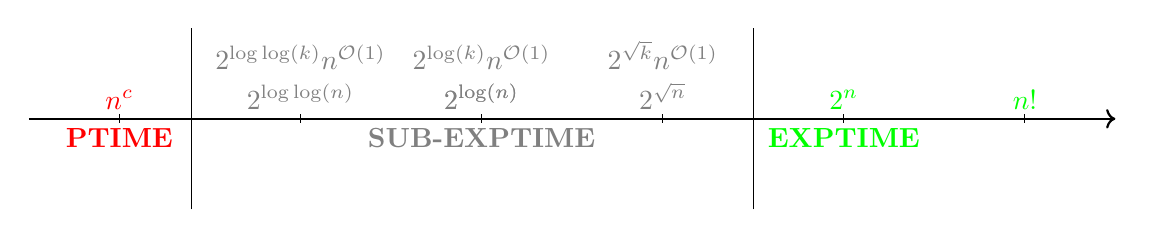
\begin{tikzpicture}[scale=1.15]
  \draw[thick, ->] (0,0) -- (12,0) node [below] {};
    \foreach \x in {1,3,...,12}
    \draw (\x, 0.05) -- node[pos=0.5] (point\x) {} (\x, -0.05);
    %\draw (\x, 0.1) -- node[pos=0.5] (point\x) {} (\x, -0.1);
    % node's content --- access them as point1...point5
    \path (point1) node [red, below] {\textbf{PTIME}};
    \draw (1.8, -1) -- node[pos=0.5] (point2) {} (1.8, 1);
    %\draw (\x, 0.1) -- node[pos=0.5] (point\x) {} (\x, -0.1);
    \path (point1) node [red, above] {\textbf{$n^c$}};
    %\path (point1) node [above] {$A=1$};
    \path (point3) node [gray, above] {\textbf{$2^{\log \log(n)}$}};
    \path (point3) node [gray, above=0.5cm] {\textbf{$2^{\log \log(k)} n^{\mathcal{O}(1)}$}};
    \path (point5) node [gray, above] {\textbf{$2^{\log(n)}$}};
    \path (point5) node [gray, above=0.5cm] {\textbf{$2^{\log(k)} n^{\mathcal{O}(1)}$}};
    \path (point5) node [gray, above] {\textbf{$2^{\log(n)}$}};
    \path (point5) node [gray, below] {\textbf{SUB-EXPTIME}};
    \path (point7) node [gray, above] {\textbf{$2^{\sqrt{n}}$}};
    \path (point7) node [gray, above=0.5cm] {\textbf{$2^{\sqrt{k}} n^{\mathcal{O}(1)}$}};
    \path (point9) node [green, above] {\textbf{$2^{n}$}};
    \path (point11) node [green, above] {\textbf{$n!$}};
    \draw (8, -1) -- node[pos=0.5] (point8) {} (8, 1);
    \path (point9) node [green, below] {\textbf{EXPTIME}};
    % you got the idea... 
  \end{tikzpicture}
\end{center}

\pause\textbf{Solution}: A new assumption based again on \textit{Hardness of SAT} 

\end{frame}

\begin{frame}[c]{Recall: q-SAT}

\end{frame}

\begin{frame}[c]{ETH and SETH}
    \begin{exampleblock}{Exponential Time Hypothesis}
    
    There is $\delta > 0$ s.t. $\mathtt{3SAT}$ can not be solved in time $\mathcal{O}(2^{\delta n})$ 
    
    \end{exampleblock}
    
    \pause\begin{exampleblock}{Strong Exponential Time Hypothesis}
    For every $\delta < 1$ there is $q$ s.t. $\mathtt{qSAT}$ cannot be solved in time $\mathcal{O}(2^{\delta n})$
    \end{exampleblock}
    
    %q-SAT inevitabily getting more difficult
    
\begin{enumerate}
%    \item $2^{\delta n} = (2^\delta)^n$: $\exists$ no algorithm solving 3SAT in $\mathcal{O}(\delta^n)$ with $\delta \leq 1$ 
    \pause\item $\mathtt{ETH} \Rightarrow \mathtt{3SAT}$ can not beat $2^{\mathcal{O}(n)}$ 
    \pause\item $\mathtt{SETH} \Rightarrow \mathtt{ETH}$ (Proof: \cite[Theorem 14.5]{Cygan2015})
    \pause\item  $\mathtt{ETH}$ is commonly believed, $\mathtt{SETH}$ still discussed.
\end{enumerate}
\end{frame}

\begin{frame}[c]{Transfering Lower Bounds by Reductions}

Observe the \textbf{Textbook} reduction(e.g. \cite{redvc}) from $\mathtt{3SAT} \leq \mathtt{VERTEX~COVER}$:

\\~

For example given: $ \phi = (x \lor y \lor \overline{z}) \land (x \lor \overline{y}) \land (\overline{x} \lor \overline{z} \lore \overline{y})$
    \begin{center}
        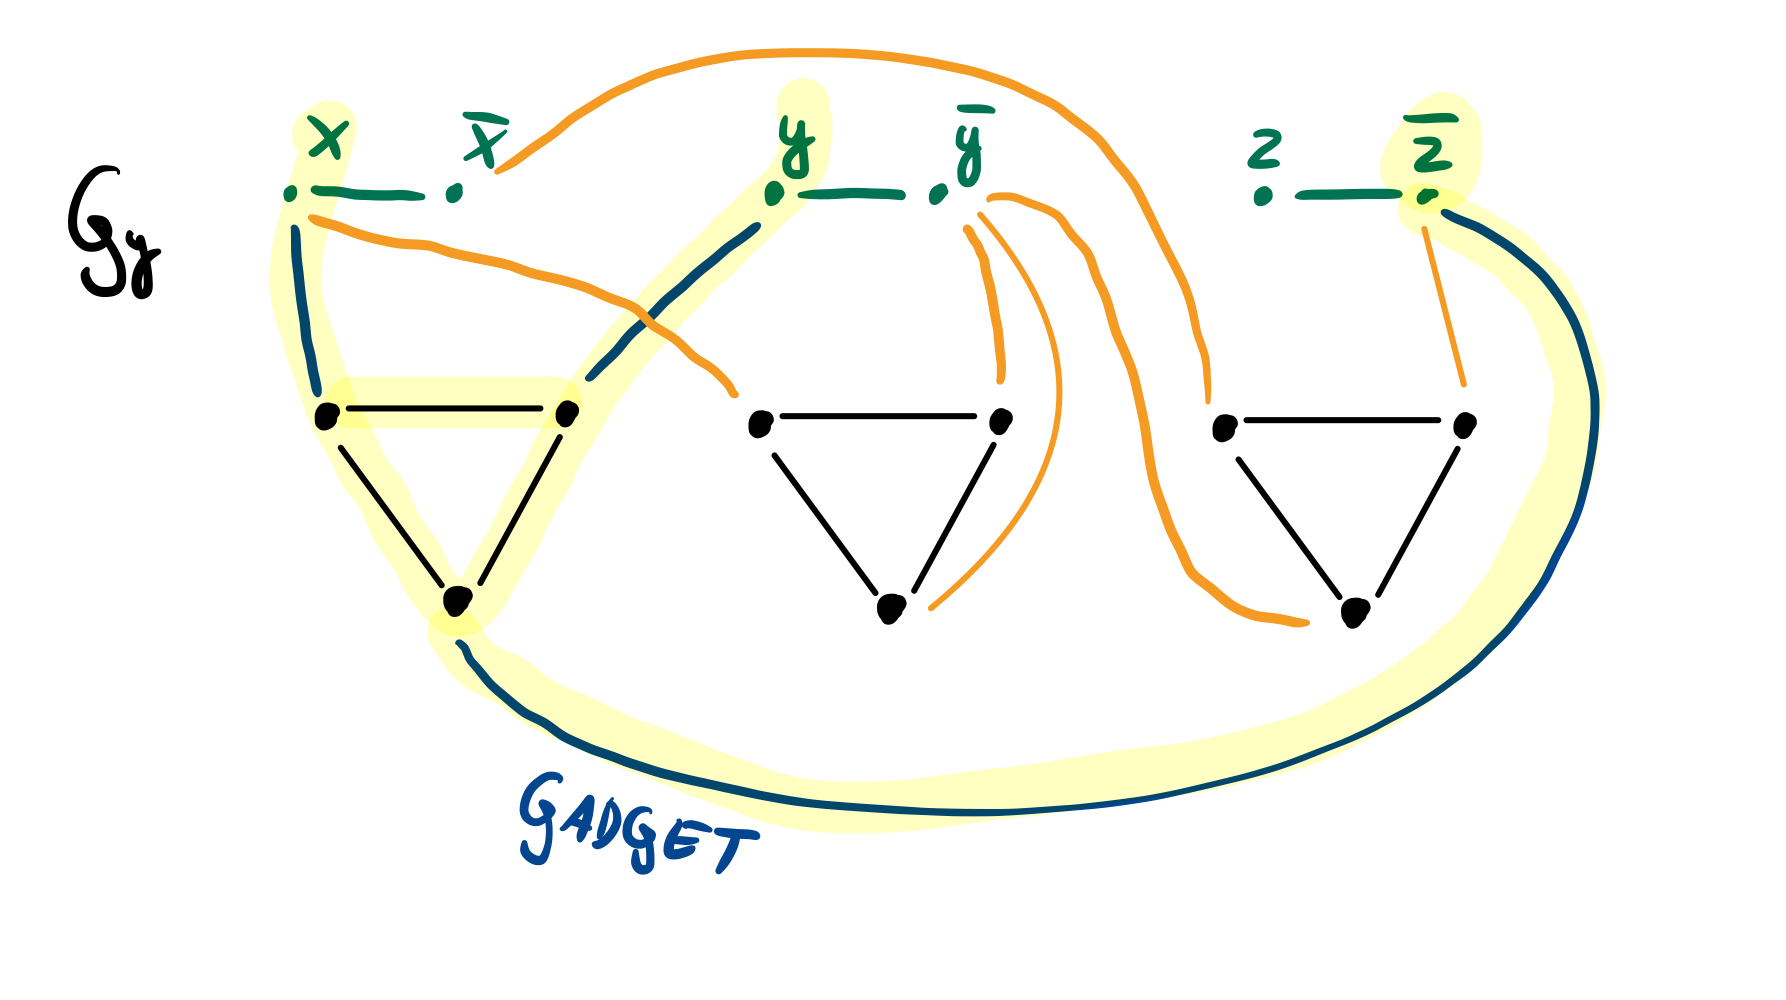
\includegraphics[scale=0.12]{img/reduce-to-VC.png}
    \end{center}
    
%\begin{block}{Observation 1}
%       Simmons Hall is composed of metal and concrete.
%\end{block} %   \begin{alertblock}{Observation 1}
\end{frame}

\begin{frame}[c]{$\mathtt{3SAT} \leq \mathtt{VERTEX~COVER}$: Analysis}
\begin{center}
$\begin{bmatrix}
   \text{Formula~} \phi \\
   n \mathtt{~Variables} \\
   m \mathtt{~Clauses} \\
\end{bmatrix} \rightsquigarrow	
\begin{bmatrix}
   \text (G, k)\\
   2n + 3m \mathtt{~Vertices} \\
   n + 6m \mathtt{~Edges} \\
   k = 2n + m
\end{bmatrix} 
$

\begin{itemize}
       \item $\#\mathtt{clauses}_{\mathtt{3SAT}} = m = \binom{N}{3} = \frac{N!}{3!(N-3!)}=\frac{N(N-1)(N-2)(N-3)!}{3!(N-3)!}=\frac{N(N-1)(N-2)}{3!}\in \mathcal{O}(n^3)$
       \item $\Rightarrow N,M \in \mathcal{O}(n^3)$
\end{itemize}
      
\pause\begin{block}{Corollary}
Assume $\mathtt{VERTEX~COVER}$ can be solved in time $2^{o(\sqrt[3]{N+M})}$

$\Rightarrow \mathtt{3SAT}$ could be solved in $2^{o(n)}$ by \textit{pipelining} the reduction. \textbf{\textcolor{red}{\text{\faBolt}}}
 Contradicting ETH
 
\end{block}

\\~ 
\begin{center}
    \pause\textbf{Nice. But can we do better?}
\end{center}
\\~ 
\end{center}
\end{frame}

\begin{frame}[c]{Towards a Tight Bound: Sparsification Lemma}

\textbf{Idea: }If we tighten $m = \mathcal{O}(n)$ in the input instance, then we would get $2^{o(N+M)}$ by the same (linear) reduction

\begin{block}{Sparsification Lemma (\cite{sparslem})}{
For all $\epsilon > 0$, there is a constant $K$ s.t. we can compute for every formula $\phi$ in $\mathtt{3CNF}$ with $n$ clauses over $k$ variables an equivalent formula $\bivee_{t=1}^t \psi_i$ where each $\psi_i$ is in $\mathtt{3CNF}$ and over the same $k$ variables and has $\leq K \cdot k$ clauses. Moreover, $t \leq 2^{\epsilon k}$ and the computation takes $\mathcal{O}(2^{\epsilon k}n^c)$ time
}
\end{block}
\textbf{Proof: } Omitted, but idea: Branching over a set of variables.
\end{frame}

\begin{frame}[c]{Turning Back to Our Reduction}
\begin{itemize}
    \item Using \textbf{Sparsification Lemma}: $\mathcal$
    \item TODO
\end{itemize}
\end{frame}

\begin{frame}[c]{More Tight Bounds For Classical Problems}

\textbf{Consequence: } Assuming ETH, there is no $2^{o(n)}$ time algorithm for

\\~
\begin{center}

\begin{itemize}
    \item $\mathtt{INDEPENDENT~SET}$
    \item $\mathtt{CLIQUE}$
    \item $\mathtt{DOMINATING~SET}$
    \item $\mathtt{VERTEX~COVER}$
    \item $\mathtt{HAMILTONIAN~PATH}$
    \item $\mathtt{FEEDBACK~VERTEX~SET}$
\end{itemize}

\end{center}
\end{frame}

\begin{frame}[c]{Consequences For Parametrized Problems}

Because ... this instantly rules out fpt.-.. for particulat

\textbf{In General: } If there is a PTIME reduction from $\mathtt{3SAT} \leq_{\mathtt{FPT}} L$, where $k \leq f(n+m)$, then assuming ETH \textbf{L cannot be solved in time $2^{o(f^{-1}(k))}\cdot poly(|x|)$}
\end{frame}

\begin{frame}[c]{Key Takeaways III}
\begin{center}
\begin{quote}
    If there would be just three things, you should take away...
\end{quote}
\begin{itemize}

\end{itemize}
\end{center}
\end{frame}

\begin{frame}[noframenumbering,plain,allowframebreaks]{References}
\begin{columns}
    \column{0.85\paperwidth}
        \printbibliography
    \end{columns}
\end{frame}

%%TODO inld
%\begin{frame}[fragile]{My First Example Grpah}
%\begin{center}
%    \begin{tikzpicture}
%        \tikzstyle{vertex}=[circle,fill=black!25,minimum %size=20pt,inner sep=0pt]
%        \tikzstyle{selected vertex} = [vertex, fill=red!24]
%        \tikzstyle{edge} = [draw,thick,-]
%        \tikzstyle{weight} = [font=\small]
%        \tikzstyle{selected edge} = [draw,line width=5pt,-,red!50]
%        \tikzstyle{ignored edge} = [draw,line width=5pt,-,black!20]
%        \begin{dot2tex}[styleonly,codeonly, circo,options=-s -tmath]
%%        digraph G {
 %       1 [style="state st,visible on=<2->,color=red"]; 
 %       2 [style="state st,visible on=<3->"]; 
 %       3 [style="state st,visible on=<4->"];  
 %       1->2 [label="1/2",style="visible on=<3->",lblstyle="visible %on=<3->"];
 %       2->3 [label="1/2",style="visible on=<4->",lblstyle="visible %on=<4->"];
 %       3->1 [label="1/2",style="visible on=<5->",lblstyle="visible %on=<5->"];
 %       }
 %   \end{dot2tex}
%\end{tikzpicture} 
%\end{center}
%\end{frame}

%\begin{frame}{Frame Title}{Subtitle}
%    \begin{block}{Observation 1}
%%        Simmons Hall is composed of metal and concrete.
%   \end{block} %   \begin{alertblock}{Observation 1}
 %       Simmons Hall is composed of metal and concrete.
 %   \end{alerblock}
 %   
 %   \begin{exampleblock}{Observation 1}
 %       Simmons Hall is composed of metal and concrete.
 %   \end{exampleblock}
%\end{frame}

%\begin{frame}{Frame Title}
%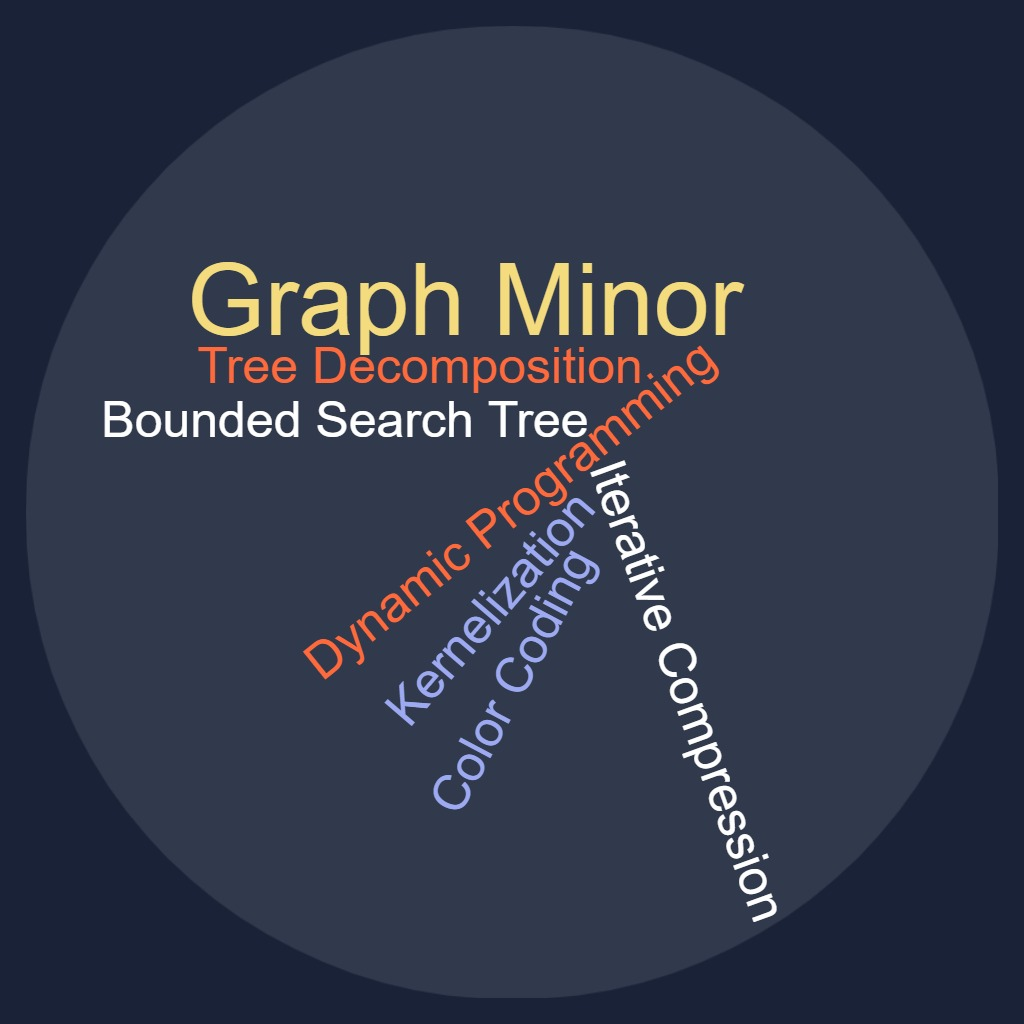
\includegraphics[]{img/wordcloud.jpg}
%\end{frame}

\end{document}
